\chapter{Ausgangssituation/IST-Analyse}
\label{Ausgangssituation/IST-Analyse}

\section{Architekturlimitationen des bisherigen Systems}

\subsection{Sequenzielle Befehlsstruktur}
\label{Sequenzielle Befehelsstruktur}
Die vorliegende Befehlsübermittlung an den Movemaster EX RV-M1 wird in der Software \textit{Objekterkennung\_RoboETH} sequenziell realisiert. \ref{sequenzielle Abfolge an Befehlen} zeigt qualitativ auf, wie eine solche Abfolge aussieht.
\begin{figure}[h!]
	\centering
	\begin{tikzpicture}[
		node distance=0cm, 
		block/.style={draw=black, thick, minimum height=0.8cm, minimum width=2.2cm, align=center},
		action/.style={block, fill=blue!20},
		wait/.style={block, fill=red!40, minimum width=2.8cm}
		]
		
		% Haupt-Thread Zeitstrahl
		\draw[thick, ->] (0,-1.5) -- (11,-1.5) node[right] {$T$};
		
		% Blöcke nebeneinander positioniert
		\node[action] (b1) at (1.1, 0) {Befehl 1};
		\node[wait, right=0cm of b1] (w1) {Thread.Sleep()};
		\node[action, right=0cm of w1] (b2) {Befehl 2};
		\node[wait, right=0cm of b2] (w2) {Thread.Sleep()};
		
		% Annotationen für T_senden (unter den Befehlen)
		\draw[<->, thick] (b1.south west) ++(0,-0.2) -- ++(2.2,0) node[midway, below] {$T_{senden}$};
		\draw[<->, thick] (b2.south west) ++(0,-0.2) -- ++(2.2,0) node[midway, below] {$T_{senden}$};
		
		% T_sleep Annotations unter den Wait-Blöcken
		\draw[<->, thick] (w1.south west) ++(0,-0.2) -- ++(3.2,0) node[midway, below] {$T_{schlafen}$};
		\draw[<->, thick] (w2.south west) ++(0,-0.2) -- ++(3.2,0) node[midway, below] {$T_{schlafen}$};
		
		% Hilfslinien von den Blöcken zum Zeitstrahl
		\draw[dashed, gray] (w1.south west) -- ++(0,-0.7);
		\draw[dashed, gray] (w1.south east) -- ++(0,-0.7);
		\draw[dashed, gray] (w2.south west) -- ++(0,-0.7);
		\draw[dashed, gray] (w2.south east) -- ++(0,-0.7);
		
	\end{tikzpicture}
	\caption{Sequenzielle Abfolge an Befehlen (Eigene Darstellung)}
	\label{sequenzielle Abfolge an Befehlen}
\end{figure}
Es ist erkennbar, dass nach jedem gesendeten Befehl ein \textit{Thread.Sleep()-Befehl} den gesamten Hauptthread für eine nicht vernachlässigbare Zeitspanne $T_{schlafen}$ blockiert. Die theoretische Zeit $T$ die benötigt wird, bis ein Befehl vollständig an den Roboter gesendet, von ihm verarbeitet und ausgeführt wird, lässt sich vereinfacht mit $T_{befehlsausfuehrung} = T_{senden} + T_{schlafen}$ beschreiben.\\
\\Während dieser Zeitspanne friert die gesamte Benutzeroberfläche sowie die Handlungsfähigkeit des Hauptthreads ein. Um die Auswirkungen der sequenziellen Befehlsbereitstellung auf die Gesamtlaufzeit und die Systemstabilität zu quantifizieren, ist eine detaillierte Analyse der Ausführungszeiten sowie der Thread-Verteilung erforderlich. Hierfür wird ein reproduzierbares Messexperiment aufgesetzt - hierzu nachfolgend mehr.\\
\\Das Ziel dieser Analyse ist die Identifikation der kritischen Pfade. Durch eine explizite Messung der Zeitstempel für den Eintritt in die Befehlsverarbeitung, die Dauer der Hardware-Kommunikation und die Verweildauer in den Wartezuständen wird der „Flaschenhals“ der synchronen Architektur isoliert. Erst durch diese messtechnische Herleitung wird transparent, an welcher Stelle die CPU-Last ungenutzt bleibt und wie sich die Thread-Auslastung sowie die Laufzeit bei einer Umstellung auf eine asynchrone Pipeline-Architektur verbessern lässt.
\subsubsection{Theoretische Limitation}
\label{Theoretische Limitation}
Wird erneut \ref{sequenzielle Abfolge an Befehlen} betrachtet, so fällt auf, dass die Zeit, welche benötigt wird, um die Koordinaten der einzelnen Objekte im Arbeitsbereich des Roboters zu berechnen, nicht eingerechnet wird. Grund hierfür ist die Annahme, dass die Berechnungszeit in beiden Fällen (sequenzielle Befehlsstruktur oder asynchrone Befehlspipeline) voraussichtlich gleich ist.\\
\\Die theoretische Gesamtlaufzeit $T_{s}$ einer Befehlssequenz lässt sich durch Summation der Befehlsausführungszeiten $T_{befehlsausfuehrung}$ bestimmen:
\begin{equation}
	T_{s} = \sum_{i=1}^{n} \sum_{j=1}^{k} T_{befehlsausfuehrung, i, j}
	\label{Summation Befehlsausführungszeiten}
\end{equation}
Einsetzen der zuvor beschriebenen Zeiten ergibt:
\begin{equation}
		T_{s} = \sum_{i=1}^{n} \sum_{j=1}^{k} (T_{senden, i, j} + T_{schlafen, i, j})
		\label{Summation Befehlsausführungszeiten mit eingesetzten Zeiten}
\end{equation}
Hierbei repräsentiert der Index $i$ das jeweilige Objekt innerhalb der Bearbeitungsreihenfolge (mit $n$ als Gesamtzahl der Objekte), während der Index $j$ die spezifische Befehlsposition innerhalb eines Manipulationszyklus angibt (mit $k$ als Anzahl der Befehle pro Objekt).\\
\\In den Gleichungen \ref{Summation Befehlsausführungszeiten} und \ref{Summation Befehlsausführungszeiten mit eingesetzten Zeiten} lässt sich die direkte Korrelation zwischen dem Parameter $n$ und der durch die Bildverarbeitungsklasse erkannten Objekte erkennen. Des weiteren wird verdeutlicht, dass die Gesamtausführungszeit einer Befehlssequenz (bestehend aus $1,...,k$ Befehlen pro Objekt) linear von der Objektanzahl $n$ und der aufsummierten Wartezeiten durch \textit{Thread.Sleep()}-Befehlen abhängt.\\
\\Bei dieser theoretischen Betrachtung wird bewusst eine Worst-Case-Abschätzung mittels der fest definierten Wartezeiten getroffen, da der vorliegende Roboter und die zugehörige Software keine Bestätigung für eine abgeschlossene Bewegung liefern. Das wird in der Software durch statische Wartezeiten (erfahrungsbasiert oder alternativ grob berechnet) kompensiert, was in der Praxis allerdings zu Einbußen der Systemeffizienz führen kann.
\subsubsection{Messexperiment}
Um die theoretisch hergeleiteten Ineffizienzen und die zeitlichen Auswirkungen der sequenziellen Befehlserteilung quantitativ nachzuweisen, wurde ein deterministisches Messexperiment aufgesetzt. Selbiges muss für Vergleichbarkeit und Bewertbarkeit auch bei nachfolgenden Erweiterungen des Systems (siehe \ref{Befehlswarteschlange für dynamischere Robotersteuerung}) zu Grunde gelegt werden.\\
\\Das Messexperiment wird mit vier Zylinderobjekten durchgeführt - die Positionen sind jeweils auf der Arbeitsunterlage markiert. Abbildung \ref{fig:messexperiment} zeigt die Anordnung der Objekte sowie die zugehörigen Objektkoordinaten.
\begin{figure}[htbp]
	\centering
	% Erstes Bild (PNG)
	\begin{subfigure}[b]{0.45\textwidth}
		\centering
		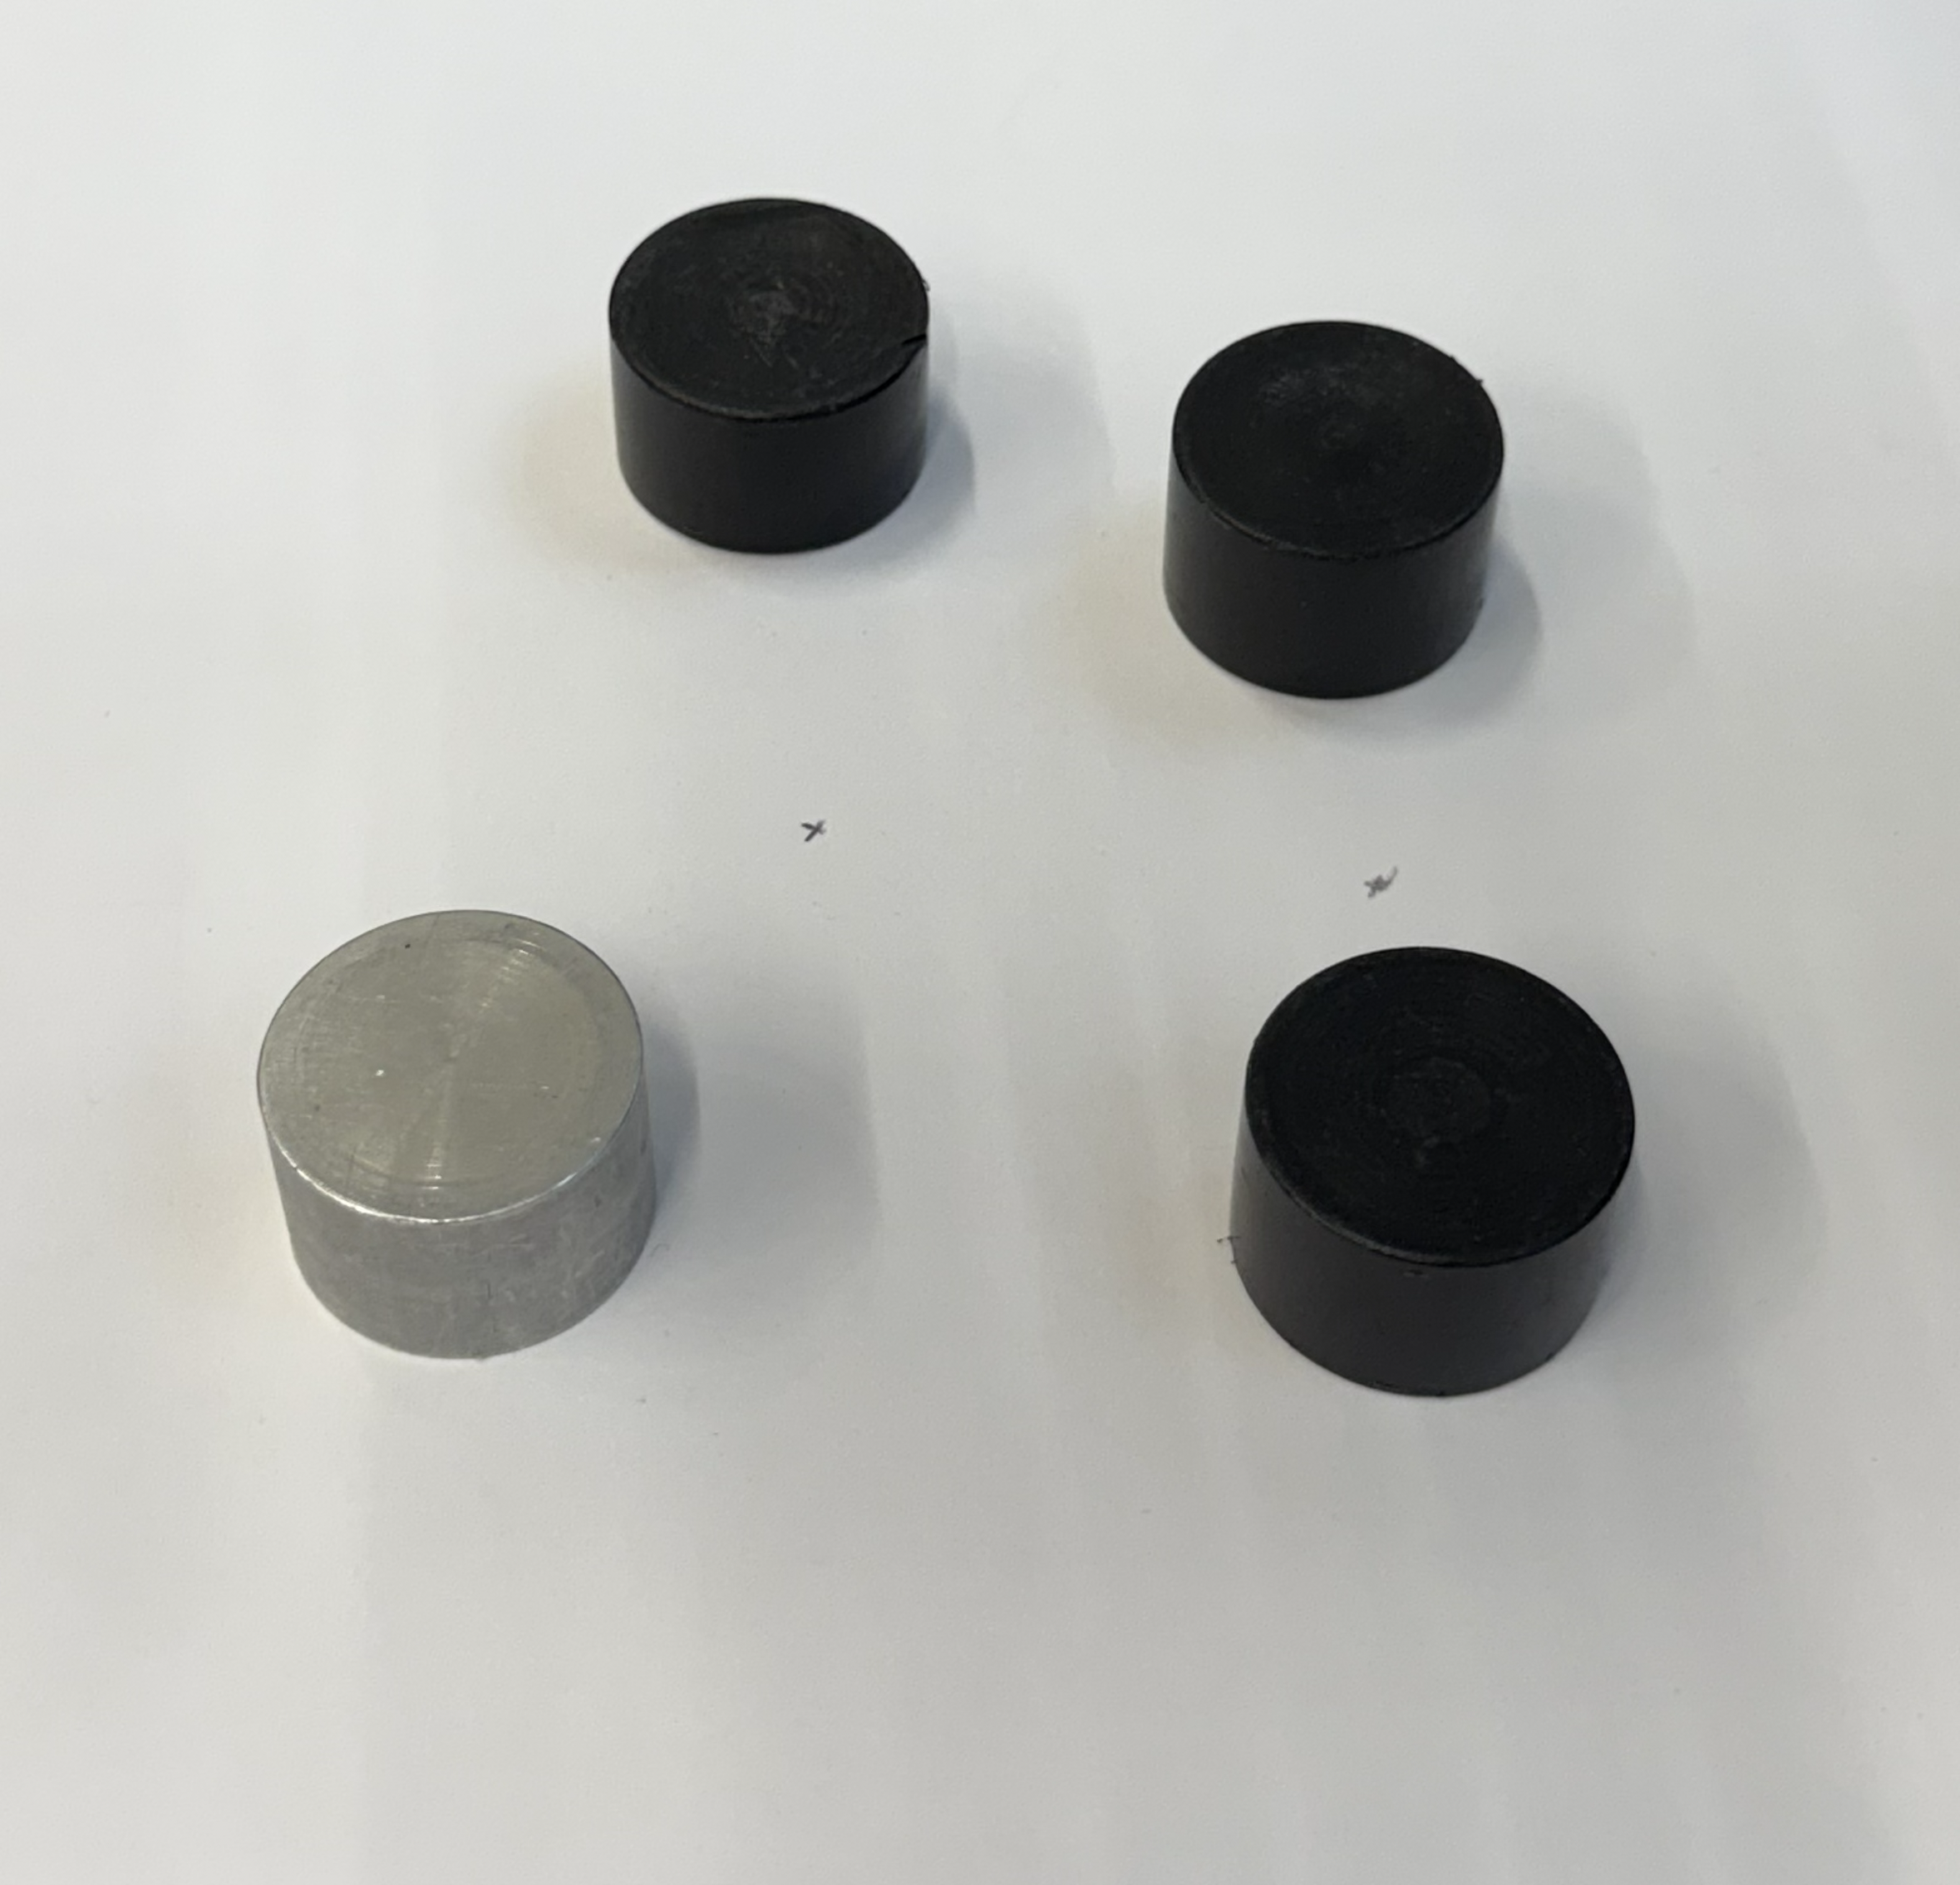
\includegraphics[width=\textwidth]{figures/Messexperiment}
		\caption{Objektanordnung}
		\label{fig:objektanordung}
	\end{subfigure}
	\hfill % Sorgt für gleichmäßigen Abstand zwischen den Bildern
	% Zweites Bild (TikZ)
	\begin{subfigure}[b]{0.45\textwidth}
		\centering
		\begin{tikzpicture}[
			box/.style={draw, minimum width=2.5cm, minimum height=0.8cm, align=center},
			greenbox/.style={box, fill=green!20},
			yellowbox/.style={box, fill=yellow!30},
			graybox/.style={box, fill=gray!30},
			node distance=0.45cm % Abstand zwischen den Boxen
			]
			
			% 5 grüne Boxen untereinander
			\node[graybox] (G0) {Objekt-ID: X-, Y-, Z-, Roll, Pitch};
			\node[greenbox, below=of G0] (G1) {Objekt 1: -42, 291, 6, -90, -8};
			\node[greenbox, below=of G1] (G2) {Objekt 2: -37, 374, 6, -90, -5};
			\node[greenbox, below=of G2] (G3) {Objekt 3: 36, 295, 6, -90, 6};
			\node[greenbox, below=of G3] (G4) {Objekt 4: 55, 346, 6, -90, 9};	
		\end{tikzpicture}
		\caption{Koordinaten im Messexperiment}
		\label{fig:koordinaten}
	\end{subfigure}
	\caption{Messexperiment zur Evaluation der Sortierperformance}
	\label{fig:messexperiment}
\end{figure}
Die Geschwindigkeit des Roboters wird per Befehl \textbf{SP} fest auf Stufe 5 (0-9 Stufen) gesetzt. Sowohl die maximalen als auch die eingestellten Geschwindigkeiten der einzelnen Achsen lassen sich aus Tabelle \ref{tab:geschwindikeiten_movemaster} entnehmen und sind für die spätere Betrachtung der inversen Kinematik des Movemaster EX RV-M1 relevant.

\begin{table}[h!]
	\renewcommand{\arraystretch}{1.2} % Etwas mehr Zeilenabstand
	\begin{tabular}{|c|c|c|}
		\hline
		\textbf{Achse} & \textbf{maximale Geschwindigkeit} & \textbf{SP5-Geschwindigkeit} \\ \hline
		Joint 1 & 120 °/sec & 29,64 °/sec \\ \hline
		Joint 2 & 72 °/sec & 17,78 °/sec\\ \hline
		Joint 3 & 109 °/sec & 26,92 °/sec \\ \hline
		Joint 4 & 100 °/sec & 24,7 °/sec\\ \hline
		Joint 5 & 163 °/sec & 40,26 °/sec\\ \hline
	\end{tabular}
	\caption{maximale bzw. SF5-Gelenkgeschwindigkeiten nach \cite[APP-52, 1-7]{rvm1manual}}
	\label{tab:geschwindikeiten_movemaster}	
\end{table}
\newpage Das Ziel, alle Objekte jeweils in einen leeren Magazinplatz zu sortieren, kann in vier Objektsortierungssequenzen und zwei Sequenzen für die Start-/Endposition eingeteilt werden. Dabei enthält jede Objektsortierungssequenz Fahr- und Greifbefehle - ersichtlich in Abbildung \ref{fig: objektsequenz}.
\begin{figure}[h!]
	\centering
	\begin{tikzpicture}[
		% Definition der Stile
		fahr/.style={rectangle, draw=blue!70, fill=blue!10, minimum height=0.8cm, minimum width=1.5cm, align=center, font=\tiny\sffamily},
		greif/.style={rectangle, draw=orange!80, fill=yellow!30, minimum height=0.8cm, minimum width=1.0cm, align=center, font=\tiny\sffamily},
		arrow/.style={-{Stealth[scale=1.2]}}
		]
		
		% --- Sequenz der Boxen ---
		\node[fahr] (B0) {Z-Offset\\Objekt\\anfahren};
		\node[fahr, right=0.2cm of B0] (B1) {Objekt\\anfahren};
		\node[greif, right=0.2cm of B1] (B2) {Greifer\\schließen};
		\node[fahr, right=0.2cm of B2] (B3) {Z-Offset\\Objekt\\anfahren};
		\node[fahr, right=0.2cm of B3] (B4) {Z-Offset\\Magazin\\anfahren};
		\node[fahr, right=0.2cm of B4] (B5) {Magazin-\\platz\\anfahren};
		\node[greif, right=0.2cm of B5] (B6) {Greifer\\öffnen};
		\node[fahr, right=0.2cm of B6] (B7) {Z-Offset\\Magazin\\anfahren};
		
		% --- Zeitstrahl ---
		\draw[arrow, thick] ($(B0.south west)-(0,0.5)$) -- ($(B7.south east)+(0,-0.5)$) node[right, font=\tiny] {Zeit $T_{objekt}$};
		
		% Verbindungsline zur Verdeutlichung der Sequenz
		\draw[dashed, gray] (B1.south) -- ++(0,-0.3);
		\draw[dashed, gray] (B7.south) -- ++(0,-0.3);
		
	\end{tikzpicture}
	\caption{Befehle innerhalb einer Objektsortierungssequenz}
	\label{fig: objektsequenz}
\end{figure}
\newline Die theoretische Gesamtverfahrzeit die der Roboter für die Sortierung aller vier Objekte benötigt, setzt sich somit zusammen aus: 
\begin{itemize}
	\item Zeit zum Erreichen der Startposition
	\item $4*T_{Objekt}$ aus \ref{fig: objektsequenz}
	\item Zeit zum Erreichen der Endposition
\end{itemize}

\newpage

\subsubsection{Praktische Limitation - Laufzeitmessung mit Simulationsexperiment}
Um die praktische Limitation der bisherigen Architektur sinnvoll beurteilen zu können, wird zunächst die theoretisch benötigte Laufzeit mit Gleichung \ref{Summation Befehlsausführungszeiten mit eingesetzten Zeiten} ermittelt.
\begin{equation*}
	T_{s} = \sum_{i=1}^{n} \sum_{j=1}^{k} (T_{senden, i, j} + T_{schlafen, i, j})
\end{equation*}
Betrachtet man den Programmcode der Klasse \textit{Roboter.cs}, so fällt auf, dass jeder Sendevorgang ($T_{senden,i,j}$) mit einem Thread.Sleep() von 800ms beaufschlagt wird. Dies geschieht, um sicherzugehen, dass der interne
\begin{table}[h!]
	\centering
	\renewcommand{\arraystretch}{1.2}
	\begin{tabular}{|c|c|c|}
		\hline
		 \textbf{Beschreibung} & \textbf{Thread.Sleep() [ms]} & $T_{schlafen,i,j}$ \\ \hline
		Fahrt auf Objekt Z-Offset  & 3000 & $T_{schlafen,i,1}$ \\ \hline
		Absenken auf Objektposition & 3000 & $T_{schlafen,i,2}$ \\ \hline
		Objekt greifen & 500 & $T_{schlafen,i,3}$ \\ \hline
		Anheben auf Objekt Z-Offset & 2000 & $T_{schlafen,i,4}$ \\ \hline
		Fahren auf Magazin Z-Offset & 5000 & $T_{schlafen,i,5}$ \\ \hline
		Absenken auf Magazinposition & 1000 & $T_{schlafen,i,6}$\\ \hline
		Loslassen des Objekts & 1000 & $T_{schlafen,i,7}$ \\ \hline
		Anheben auf Magazin Z-Offset & 1000 & $T_{schlafen,i,8}$ \\ \hline
		\textit{Anheben auf Magazin Z-Offset} & 1000 & $T_{schlafen,i,9}$ \\ \hline
	\end{tabular}
	\caption{Tabellarische Übersicht der Thread.Sleep()-Verzögerung pro Objektsequenz}
	\label{tab:thread.sleep()-zeiten}
\end{table} 
\newline Setzt man nun die ermittelten statischen Werte aus Tabelle \ref{tab:thread.sleep()-zeiten}, die Wartezeiten bei jedem Senden sowie die Zeit für Start- und Endposition in die Gleichung für die Gesamtdauer $T_{S}$ ein:
\begin{equation}
	T_{S} = 	T_{s} = 2*(1800ms) \sum_{i=1}^{4} \sum_{j=1}^{9} (T_{senden, i, j} + T_{schlafen, i, j})
\end{equation}
so erhält man eine berechnete Gesamtdauer von 



\begin{table}[h!]
	\renewcommand{\arraystretch}{1.2} % Etwas mehr Zeilenabstand
	\begin{tabular}{|c|c|c|}
		\hline
		\textbf{Objekt-ID} & \textbf{Theoretische Zeit $T_S$ [s]} & \textbf{Gemessene Zeit $T_{mess}$ [s]} \\ \hline
		Startposition & 1,8 & 24,97 \\ \hline
		Objekt 1 & 17,5 & 24,97 \\ \hline
		Objekt 2 & 17,5 & 24,91 \\ \hline
		Objekt 3 & 17,5 & 24,95 \\ \hline
		Objekt 4 & 17,5 & 24,89 \\ \hline
		Endposition & 1,8 & 24,97 \\ \hline
		\textbf{Mittelwert} & \textbf{17,5} & \textbf{24,93} \\ \hline
		\textbf{$T_{S}$} & \textbf{70} & \textbf{103,73} \\ \hline
	\end{tabular}
	\caption{Vergleich der theoretischen Laufzeit $T_S$ mit den gemessenen Werten $T_{mess}$}
	\label{tab:laufzeitanalyse_ist}
\end{table}

